\documentclass[aspectratio=43,11pt]{beamer}
\usepackage[utf8]{inputenc}
\usepackage{caption}
\usepackage{makecell}
\usepackage{framed}
\usepackage{listings}
\usepackage{csquotes}
\usepackage{mathtools}
\usepackage{hyperref}
\usepackage{graphicx}   
\usepackage{amsmath,amssymb}
\usepackage[magyar]{babel}

\usetheme{realtimeweb}

\makeindex
\graphicspath{ {figs/} }

\lstdefinelanguage{JavaScript}{
  keywords={typeof, new, true, false, catch, function, return, null, catch, switch, var, if, in, while, do, else, case, break, await, async, const, let},
  keywordstyle=\color{blue}\bfseries,
  ndkeywords={class, export, boolean, throw, implements, import, this},
  ndkeywordstyle=\color{darkgray}\bfseries,
  identifierstyle=\color{black},
  sensitive=false,
  comment=[l]{//},
  morecomment=[s]{/*}{*/},
  commentstyle=\color{purple}\ttfamily,
  stringstyle=\color{red}\ttfamily,
  morestring=[b]',
  morestring=[b]"
}

\lstset{basicstyle=\ttfamily,
  showstringspaces=false,
  commentstyle=\color{red},
  keywordstyle=\color{blue}
}

\captionsetup[figure]{labelformat=original}
\setlength{\belowcaptionskip}{0.25cm}
\setlength{\abovecaptionskip}{0.25cm}

\definecolor{graycolor}{gray}{0.96}

\setbeamerfont{section number projected}{family=\rmfamily,series=\bfseries,size=\normalsize}
\setbeamercolor{section number projected}{bg=graycolor,fg=Blue}
\setbeamercolor*{item}{fg=Blue}
\setbeamercolor{block title}{fg=Blue,bg=graycolor}
\setbeamercolor{caption name}{fg=Blue}
\setbeamercolor{bibliography entry author}{fg=Blue}
\setbeamercolor{bibliography entry location}{fg=Blue} 
\setbeamercolor{bibliography entry note}{fg=Blue}  
\setbeamertemplate{footline}[frame number]
\setbeamertemplate{caption}[numbered]
\setbeamertemplate{navigation symbols} {} 
\setbeamertemplate{bibliography item}{\insertbiblabel}
\setbeamertemplate{footline}[frame number]
\setbeamertemplate{caption}[numbered]
\setbeamertemplate{frametitle continuation}{}

\title{Projekt Bemutató}
\subtitle{Community Space - A place for all your memos}
\author{Lukács Zsolt}

\begin{document}

\frame{\titlepage}

\section{CS Bevezető}

\begin{frame}
    \frametitle{Bevezető és CS projekt hatóköre}

    Tudásmegosztásra kihelyezett közösségi munkaplatform a vállalati/egyéb közösségen belüli gyors információmegosztásra és megőrzésre rövid memo-k formájában, ahol bárki könnyedén megoszthatja aktuális gondolatait/felhívásait/közléseit egy adott tematikáról vagy gondolatról csoportokon belül, amelyeket mások teljesíthetnek és elvégzésüket kvázi kötelezővé tehetik határidők megadásával, amelyekre a felhasználók értesítést kapnak sok más egyéb mellett.

    \medbreak

    \begin{block}{Megjegyzés}
        Hub több memo-t foglal magába és tagok csoportjaként fogható fel, a memo egy általában rövid üzenet, amely hasonlít az e-mail-hez, gyakran valamilyen elvégzendő feladatot fog meghatározni.
    \end{block}
\end{frame}

\begin{frame}
    \frametitle{Bevezető és CS projekt hatóköre}

    Alapvető funkcionalitások és üzleti folyamatok:
    \begin{itemize}
        \item Felhasználók képesek contókat létrehozni a platformhoz való csatlakozáshoz;
        \item Saját közösségeket, hub-okat létrehozni, meglévőkhöz csatlakozási kérelmeket leadni, tagokat adminisztrátor felhasználók menedzselhetik;
        \item Felhasználók képesek memo-kat megosztani különböző láthatósági szintekkel, prioritásokkal és határidővel kizárólag a hub-on belül, ezek elolvasni, módosítani, archívumba helyezni, törölni, kitűzni, teljesíteni, keresni közöttük, stb.;
        \item Aktivitási hőtérkép és interakciós (milyen tevékenységek végződtek el a múltban) listázás az aktuális hétre vetítve;
        \item Felhasználók képesek összegzés formájában megtekinteni az összes hub-jukat, informálódni arról, hogy hány új memo van, hány aktív tag, stb.;
        \item \textbf{Real-time} értesítési mechanizmus, platformbéli aktív felhasználók kilistázása.
    \end{itemize}

    \begin{block}{Megjegyzés}
        Egyéb kiegészítő (technikai) funkcionalitások az automatizált \texttt{GitLab CI/CD}, a felhő \texttt{K8S}, annak menedzsmentje \texttt{Terraform}-al, és a \texttt{Helm Chart} kitelepítés.
    \end{block}
\end{frame}
\section{CS Architektúra}

\begin{frame}
    \frametitle{CS Architektúra}

    \begin{center}
        Rendszer alapvető központi entitásai: felhasználók, hub-ok, memo-k (kiegészítőleg aktivitások és értesítések).
    \end{center}

    \begin{figure}[htbp]
        \centering
        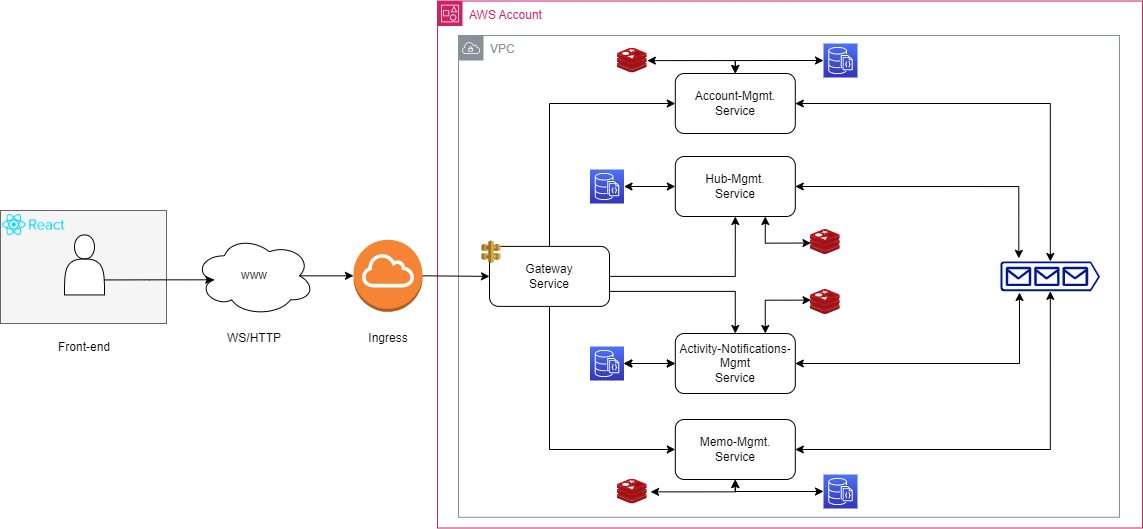
\includegraphics[width=1\textwidth]{arch}
        \caption{CS architektúra és komponens diagram}
    \end{figure}

    \begin{center}
        Micro-service architektúra összesen (jelenleg) 5 szolgáltatással.
    \end{center}
\end{frame}
\section{CS Technológiai Stack}

\begin{frame}
    \frametitle{CS Technológiai Stack}

    Front-end összefoglaló:
    \begin{itemize}
        \item Nyelv: \texttt{Typescript};
        \item Keretrendszer: \texttt{Next.js};
        \item Komponenskönyvtár: \texttt{MaterialUI}.
    \end{itemize}

    \medbreak

    Back-end összefoglaló:
    \begin{itemize}
        \item NoSQL adatbázis: \texttt{MongoDB};
        \item Cache megoldás: \texttt{Redis};
        \item Általános back-end keretrendszer: \texttt{Spring Boot} (micro-service-k implementálására, pl. \texttt{Spring JPA, Spring Repository, Spring WebFlux});
        \item Üzenet broker (in-cluster): \texttt{Kafka};
        \item Infrastruktúra és DevOps: \texttt{Terraform} (K8S cluster létrehozása DigitalOcean-on), \texttt{K8S és Helm} és \texttt{GitLab CI/CD}.
    \end{itemize}

    \medbreak

    Kiegészítő egyéb technológiák: \texttt{WebSocket} és \texttt{Socket.IO}, \texttt{Spring Gateway}, \texttt{useSWR} adat pulling-hoz, stb.

\end{frame}
\section{CS Architektúra Magyarázat}

\begin{frame}
    \frametitle{CS Architektúra Magyarázat}

    \begin{itemize}
        \item Back-end egyetlen belépési pontja a \texttt{Gateway} szolgáltatás (HTTP/WebSocket), általános routing a többi szolgáltatáshoz; egyetlen \texttt{K8S Ingress}-t kitéve.
        \item Minden szolgáltatás külön \texttt{Mongo} adatbázissal rendelkezik és a legtöbb hívásukat cache-lik \texttt{Redis}-ben.
        \item A szolgáltatások soha nem kommunikálnak HTTP-n keresztül, kizárólag Kafka consumer-producer topic-okon keresztül, amelyeknek több szerepe is van:
              \begin{enumerate}
                  \item Amennyiben egyik szolgáltatás működése függ a másik szolgáltatásban tárolt adatoktól, a második szolgáltatásnak kötelessége egy topic-on keresztül közzé tenni ezeket a változásokat (i.e., legtöbb adatbázisváltozás valamilyen formában egy topic-ra közzé lesz téve, hogy a többi szolgáltatás erre hallgasson és a saját adatbázisába mentse el az adatokat), így függetlenné téve őket egymástól.
                  \item Az \texttt{Activity-Notifications-Mgmt.} a platformbéli aktivitásokat üzenetsoron keresztül fogadja a többi szolgáltatástól, ezeket értesítésekké üzenetsoron keresztül teszi (az aktivitási üzenet fogadása után egy újabb üzenetet küld önmagának az értesítést kiküldésére/kezelésére).
                  \item A memo teljesítési emlékeztetők üzenetsoron keresztül kerülnek load-balance-lésre az \texttt{Activity-Notifications-Mgmt.} példányok között (periodikusan megnézi melyek a még nem teljesített, de sürgős memo-k és üzeneteket tesz közzé minden memo-nak, amiben értesíti azokat a felhasználókat, akik még nem teljesítették az adott memo-t).
              \end{enumerate}
    \end{itemize}
\end{frame}

\begin{frame}
    \frametitle{CS Valósidejűség}

    (Jelenleg) Két \texttt{WebSocket}-en (valójában \texttt{Socket.IO}-n, Netty bázisú szerverrel) alapuló valósidejű folyamat:
    \begin{enumerate}
        \item online státusz, értsd. aktív felhasználók;
        \item értesítések (egyéni vagy csoportos).
    \end{enumerate}

    Megvalósítások:
    \begin{enumerate}
        \item Az online státuszért az \texttt{Account-Mgmt.} (\textit{StatusListener.java}) felel, fogadja a \texttt{Socket.IO} egy adott endpoint-jára érkező csatlakozásokat/kilépéseket karbantartva az aktív listát, amit \texttt{Redis}-ben tárol, minden változásra közölve az új listát a felhasználóknak; minden csatlakozott kliensnek periodikusan felelőssége közölni jelenlétét egy üzenet formájában (\textit{PresenceContext.tsx}); minden 1 percben újraértékeli az aktív listát, törölve azokat, akik 1 perce nem közöltek magukról semmit.
        \item Az értesítésekért az \texttt{Activity-Notifications-Mgmt.} felel (\textit{NotificationListener.java}), minden felhasználó belépéskor \texttt{RestAPI}-val lekéri az adatbázisba mentett értesítéseit, és \texttt{WS}-n keresztül fogadja az újakat; az egyéni/csoportos izoláció \texttt{Socket.IO room}-okon keresztül van megoldva.
    \end{enumerate}

    \begin{block}{Megjegyzés}
        Minden \texttt{Socket.IO} interakció token-t igényel.
    \end{block}
\end{frame}
\section{Zárószó}

\begin{frame}
    \frametitle{Zárószó}

    A kód megtalálható a \href{https://gitlab.com/rockdonald2/community-space}{gitlab.com/community-space} oldalon.

    \medbreak

    Ahol a kód 3 részben van szétbontva:
    \begin{itemize}
        \item \texttt{backend/} mappa tartalmazza a projekt micro-service-einek kódját, jelenleg 5 ilyen projekt van ezen belül (4 service + 1 library, mind \texttt{Java Spring}-ben);
        \item \texttt{frontend/} mappa tartalmazza a \texttt{NextJS} front-end kódot;
        \item \texttt{devops/} mappa tartalmazza a \texttt{Terraform}, \texttt{Helm}, és \texttt{CI/CD} kódrészleteket, amelyek megvalósítják a folyamatos fejlesztést és kitelepítést (minden commit után automatikus build és Docker deploy folyamatok a projekt \texttt{Gitlab Registry}-jére), infrastructure-as-code a K8S cluster létrehozásához és \texttt{Helm Chart} a könnyű K8S kitelepítésért.
    \end{itemize}

\end{frame}

\end{document}
